% ----- formatovani dokumentu -----------------------------------------------
\documentclass[12pt,a4paper,titlepage,final]{report}
\usepackage[utf8]{inputenc}
\usepackage[T1, IL2]{fontenc}
\usepackage{graphicx}
\usepackage{epstopdf}
\usepackage[margin=2cm]{caption}
\usepackage[top=2cm, left=2cm, right=2cm, text={17cm, 24cm}, ignorefoot]{geometry}
\usepackage[usenames,dvipsnames]{color}
\usepackage{url}
\usepackage{setspace}
\singlespacing
\usepackage[square, numbers]{natbib} 
\pagestyle{plain}
\pagenumbering{arabic}
\setcounter{page}{1}
\setcounter{secnumdepth}{-1}
\setlength{\parindent}{1cm}	
\usepackage{natbib}


% ----- vyberte jazyk -------------------------------------------------------
\usepackage[english,czech]{babel}
%\usepackage[english]{babel}

% ----- dopiste titulky -----------------------------------------------------
\newcommand\Course{Analýza a návrh informačních systémů}
\newcommand\WorkTitle{Firma2}
\newcommand\AuthorA{Michal Riša}
\newcommand\AuthorAEmail{xrisam01@stud.fit.vutbr.cz}
\newcommand\AuthorB{Pavel Macenauer}
\newcommand\AuthorBEmail{xmacen02@stud.fit.vutbr.cz}
\newcommand\Faculty{Fakulta Informačních Technologií}
\newcommand\School{Vysoké Učení Technické v Brně}

\usepackage[
pdftitle={\WorkTitle},
pdfauthor={\AuthorA, \AuthorB},
bookmarks=true,
colorlinks=true,
breaklinks=true,
urlcolor=blue,
citecolor=blue,
linkcolor=blue,
unicode=true,
]
{hyperref}


%%%%%%%%%%%%%%%%%%%%%%%%%%%%%%%%%%%%%%%%%%%%%%%%%%%%%%
%----------------- TITULNÍ STRANA -------------------%
%%%%%%%%%%%%%%%%%%%%%%%%%%%%%%%%%%%%%%%%%%%%%%%%%%%%%%

\begin{document}
	\begin{titlepage}
	\begin{center}
		\includegraphics[height=5cm]{img/logo.eps}
	\end{center}
	\vfill
	\begin{center}
		\begin{Large}
			\Course\\
		\end{Large}
		\bigskip
		\begin{Huge}
			\WorkTitle\\
		\end{Huge}
	\end{center}
	\vfill
	\begin{center}
		\begin{large}
			\today
		\end{large}
	\end{center}
	\vfill
	\begin{flushleft}
		\begin{large}
			\begin{tabular}{lll}
				Autoři: & \AuthorA, & \url{\AuthorAEmail} \\
				        & \AuthorB, & \url{\AuthorBEmail} \\
				& & \\
				& \Faculty \\
				& \School \\
			\end{tabular}
		\end{large}
	\end{flushleft}
\end{titlepage}		
	
%%%%%%%%%%%%%%%%%%%%%%%%%%%%%%%%%%%%%%%%%%%%%%%%%%%%%%
%--------------------- OBSAH ------------------------%
%%%%%%%%%%%%%%%%%%%%%%%%%%%%%%%%%%%%%%%%%%%%%%%%%%%%%%
	
\tableofcontents

%%%%%%%%%%%%%%%%%%%%%%%%%%%%%%%%%%%%%%%%%%%%%%%%%%%%%%
%---------------- PRVOTNÍ ANALÝZA -------------------%
%%%%%%%%%%%%%%%%%%%%%%%%%%%%%%%%%%%%%%%%%%%%%%%%%%%%%%

	\chapter{Prvotní analýza a plán projektu}
	
	\section{Neformální specifikace}
	Cílem projektu je navrhnout jednoduchý informační systém pro firmu organizující kursy orientované na programové vybavení počítačů, který ji umožní spravovat termíny kursů a zpracovávat přihlášky zákazníků.
	
	Kursy probíhají v pronajatých prostorech o různých kapacitách za vedení externích lektorů v různé termíny. Systém by tak měl zahrnovat možnost vypisovat kursy a k nim vytvořit prezentační (informační) stránku, ze které zákazník vyčte potřebné informace o kursu. Ke každému kurzu se budou vypisovat termíny a termínům přiřazovat cena, místo konání a lektor. Všechny tyto nastavení bude možno nadále i měnit.
	
	Součástí systému je i rozhraní, které umožní zákazníkům se přihlašovat na termíny. Každá přihláška bude mít jedinečný identifikátor, přes který bude možnost ji dohledat nebo spravovat. Po přihlášení se bude přihláška postupně zpracovávat pomocí daného protokolu mezi zákazníkem a zaměstnancem (přihlášení - potvrzení/odmítnutí - zaplacení - potvrzení platby).
	
	Systém by měl umožňovat správu uživatelů a změnu rolí jednotlivých uživatelů - lektor, zaměstnanec, administrátor. Tuto možnost bude mít pouze administrátor. Zákazníci nebudou mít uživatelské role a v systému budou evidování pomocí svých přihlášek.
	
	Zaměstnanec bude moci kdykoliv uzavřít nebo naopak otevřít přihlašování. I po zpracování přihlášky bude možnost měnit její stav, tzn. vyřadit ji z termínu nebo vrátit/zrušit platbu.
	
	Zákazníci budou mít možnost zažádat o vypsání konkrétního termínu nebo i kursu. Tato součást systému bude řešena jako komunikační kanál mezi žádajícím a zaměstnancem.
	
	Pro snadnou organizaci kurzů se budou jednotlivé termíny kursů zobrazovat v kalendáři, který si budou moci uživatelé systému zobrazit. Úroveň detailu kalendáře bude záviset na konkrétní roli uživatele.
	
	Systém bude implementován jako webová aplikace, která bude komunikovat s databázovým serverem. Bude se skládat ze 2 součástí - front-end (přes který se budou přihlašovat zákazníci s důrazem především na přehlednost, jednoduchost a visuální stránku věci)
a back-end (přes který se budou spravovat přihlášky, termíny, kursy, uživatelé a mj. zde najdeme zde i kalendář).

\newpage

% ----------- analyza pozadavku -----------

	\section{Analýza požadavků}
	Z neformální specifikace plynou následující požadavky:
	
	\subsection{Aktéři}		
	
		\begin{itemize}
			\item Uživatel: není přihlášen nebo evidován v systému, má možnost přihlašovat se na termíny kurzů a upravovat svou přihlášku přes její jedinečný identifikátor.
			\item Lektor: externista, který fyzicky vede kurzy, nemá práva jakkoliv zasahovat do organizace nebo vedení firmy, ale měl by být informován kdy, kde, koho a co vyučovat.
			\item Zaměstnanec: zaměstnanec firmy, který má na starosti veškerou správu plateb, kursů, termínů. Vypisuje tedy nové kursy a termíny, potvrzuje přihlášky a vykonává tak veškerou administrátorskou činnost spojenou s během firmy.
			\item Admin: vytváří a spravuje uživatele. Má přístup k citlivým částem informačního systému.
			\item Čas: reprezentuje autonomní/pravidelné činnosti systému, které se provádějí buď jako reakce na nějakou činnost jednoho z aktérů a nebo pravidelně
		\end{itemize}
		
	Využití vzájemné dědičnosti všech aktérů je výhodné především pro jednoduchost a přehlednost implementace, kdy každý aktér s vyššími právy bude vždy umět o něco více a nebudeme tak muset dělit aplikaci na části, které některý z uživatelů může používat, další ne a naopak, což zvyšuje složitost.
		
		
% ----------- use case -----------
				
	\subsection{Diagram případů použití}
	
Nasledujúci diagram prípadov použitia prehľadne zobrazuje prípady použitia asociované s vyššie uvedenými aktérmi.
		\begin{center}
			\captionsetup{type=figure}
			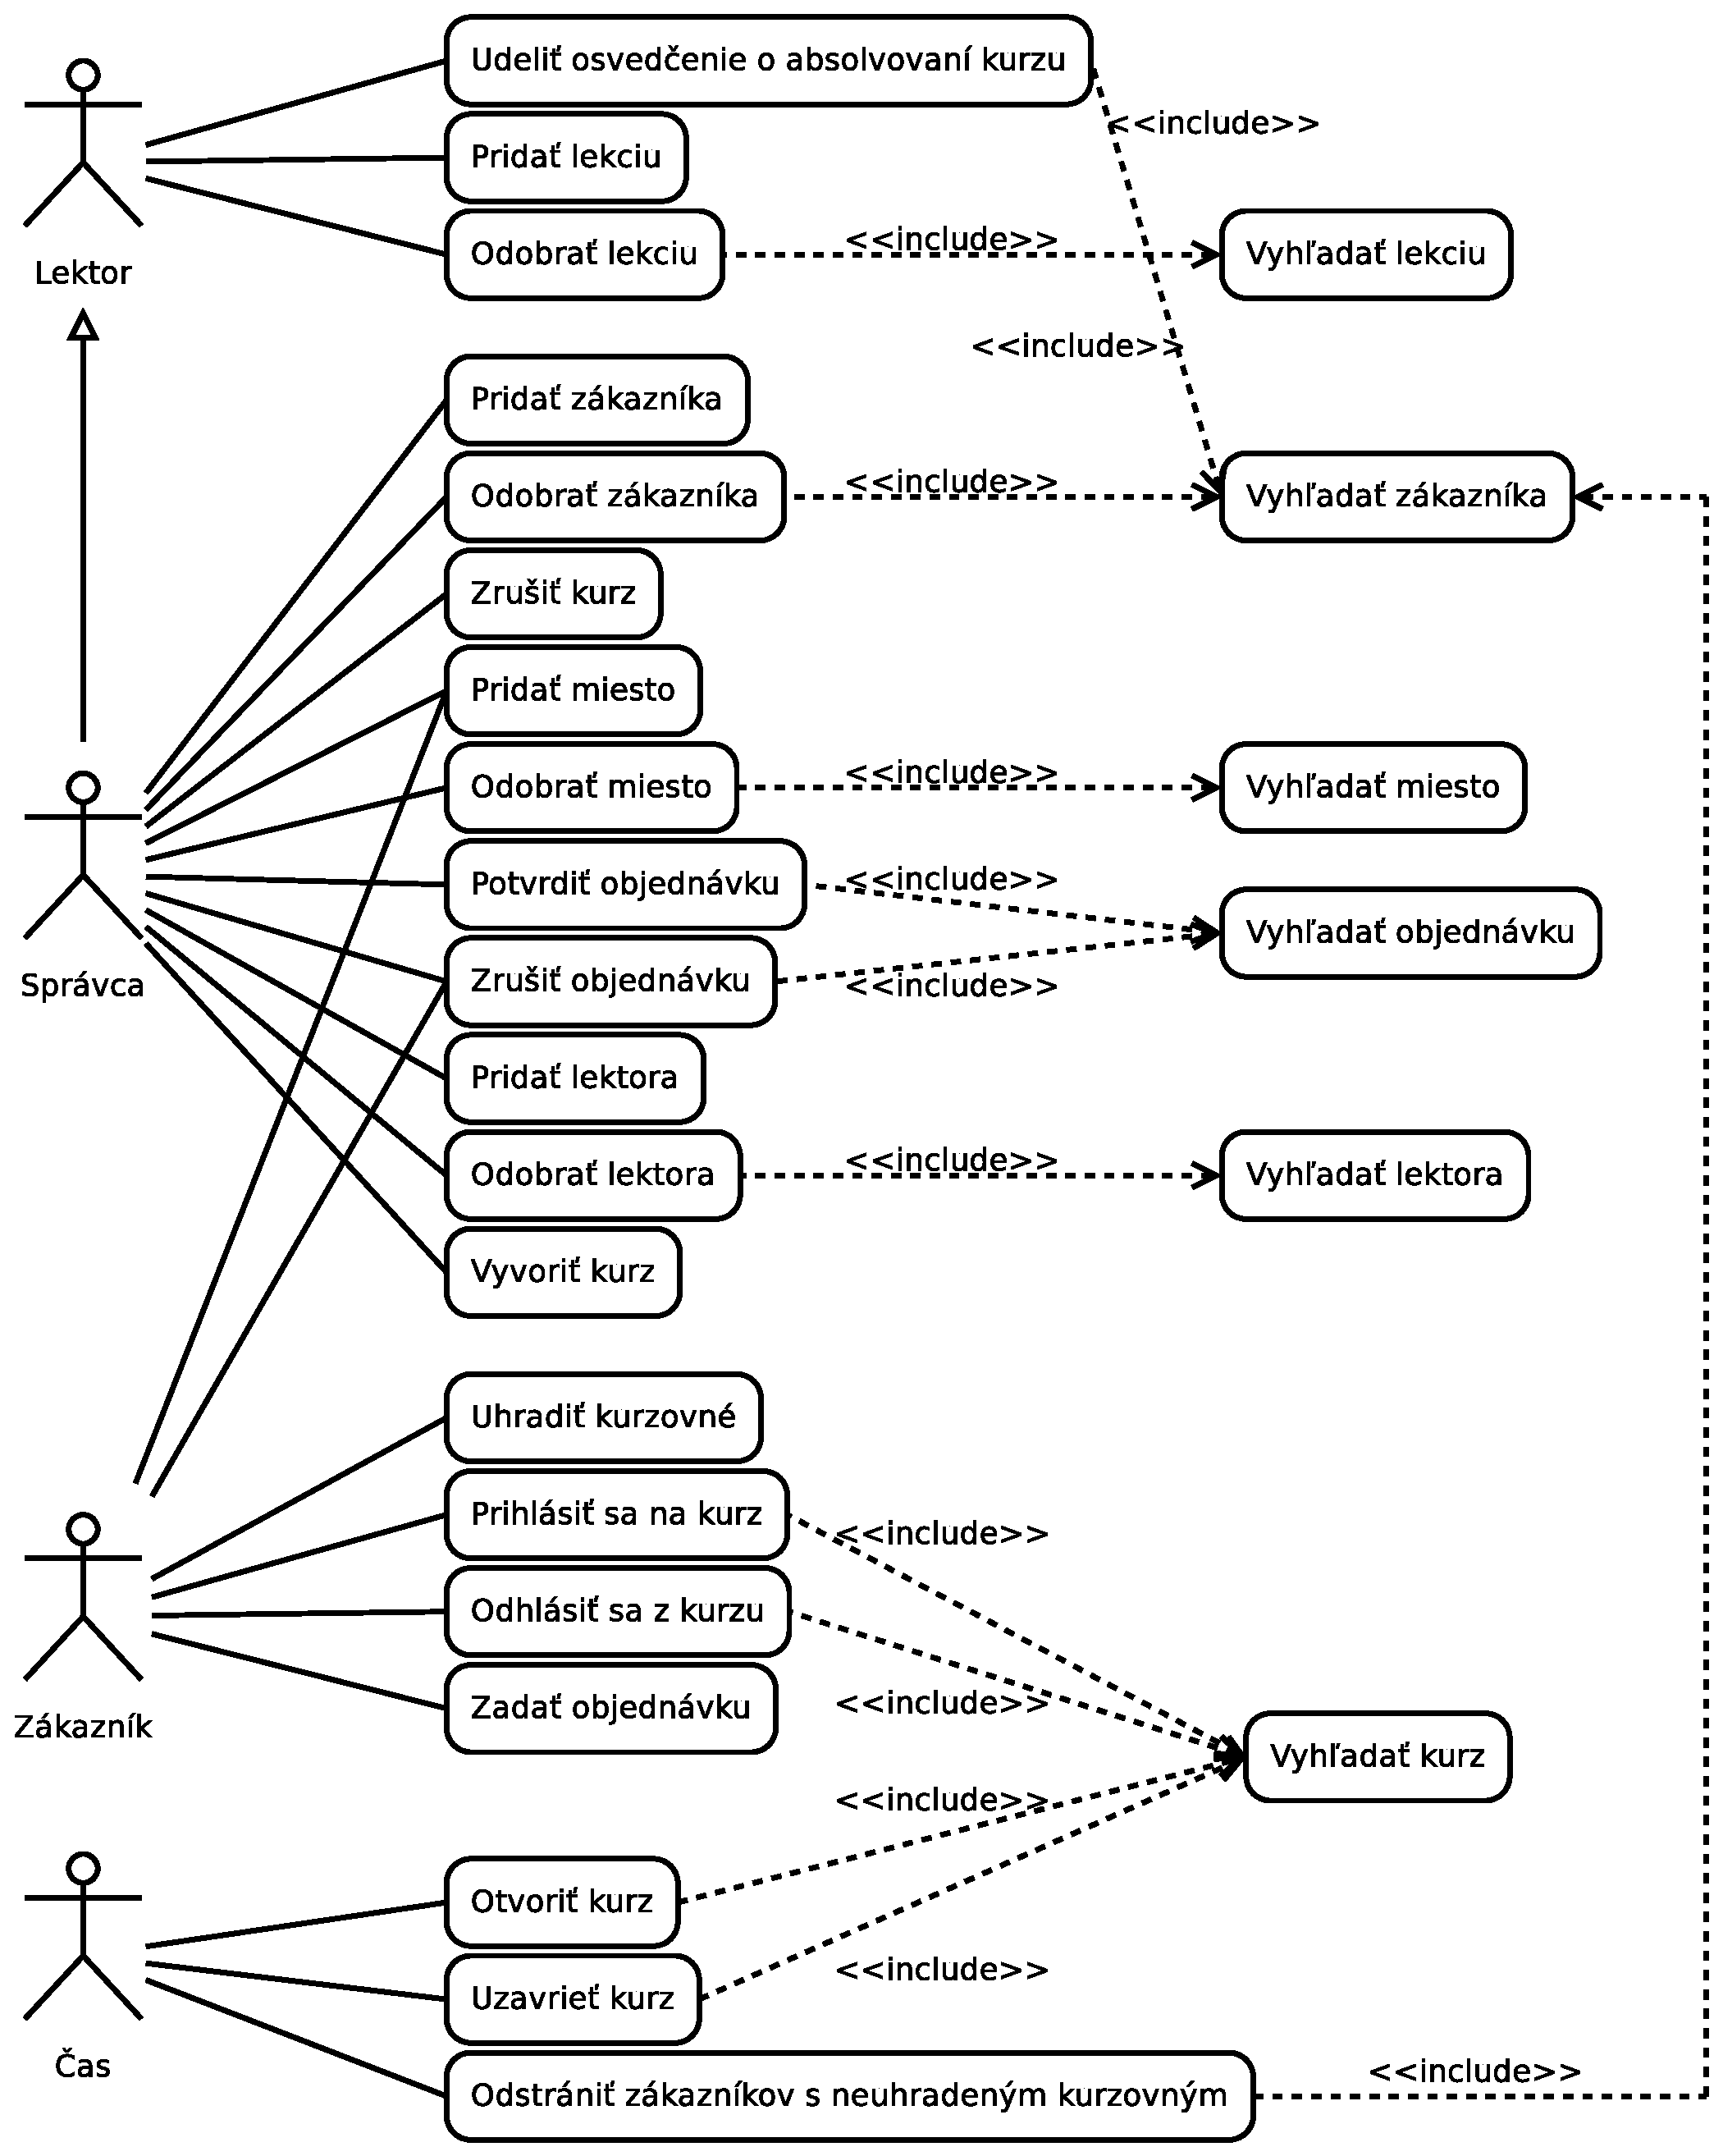
\includegraphics[height=14cm]{img/use_case.eps}
			\captionof{figure}{Kompletní diagram případů použití.}
		\end{center}
		
	\subsection{Plán projektu}
	
Na základě analýzy projektu jsme se rozhodli rozdělit projekt na 4 iterace. V prvních 2 se vytvoří prototypy obsahující drtivou většinu funkcí celého systému. Následně ve 3. iteraci se projekt překlopí již na konečnou implementaci a ve 4. se budou dodělávat funkčnosti usnadňující práci se systémem a zvyšující jeho přehlednost.
	
Prototypování po prvních 2 iteracích nám umožní zhodnotit použitelnost systému dříve, než začne být implementována ostrá verze a pomůže ve shodě se zákazníkem.
	
	\subsubsection{1. iterácia}
		\begin{center}
			\captionsetup{type=figure}
			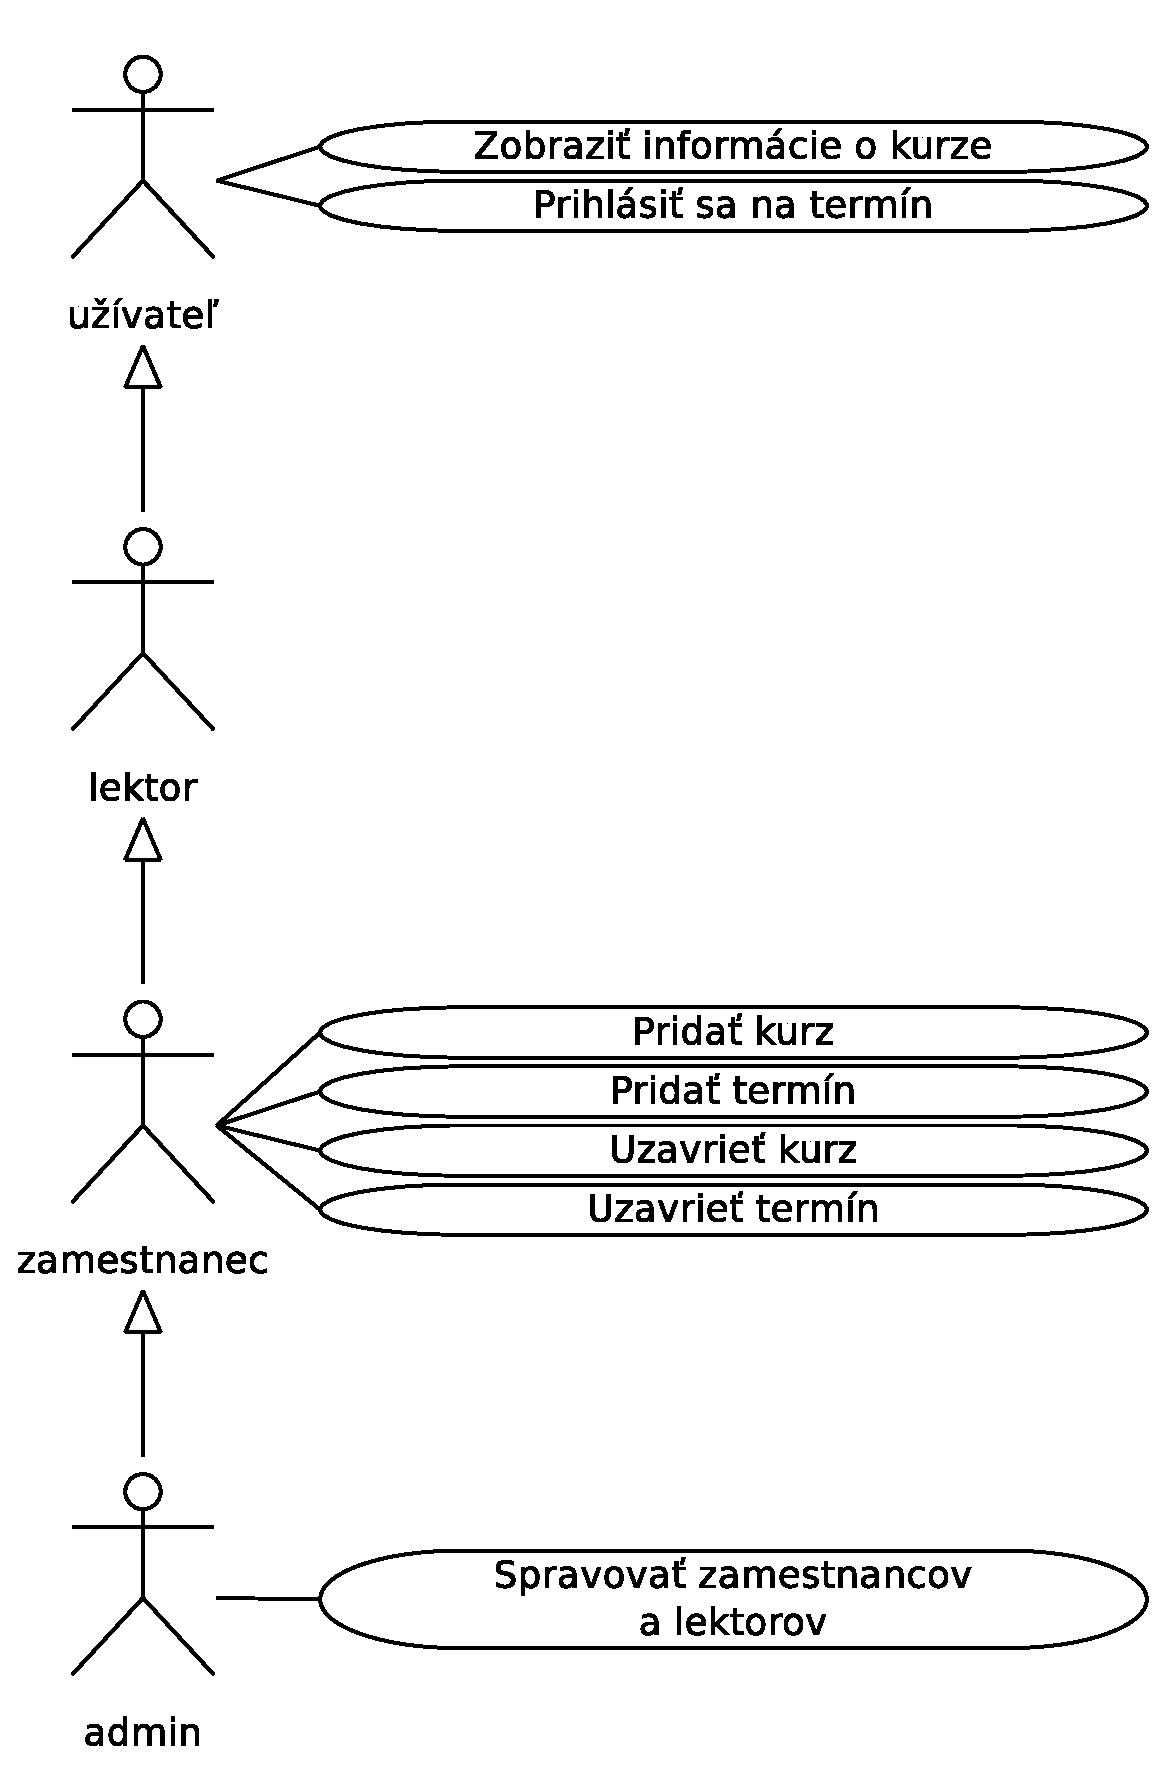
\includegraphics[height=17cm]{img/use_case_iter1.eps}
			\captionof{figure}{Diagram implementovaných případů použití po 1. iteraci.}
		\end{center}
		
Prototyp aplikace bude umět základní správu kurzů a termínů - přidávat a uzavírat kurzy a termíny. Zároveň bude umět přidávat přihlášky a vytvářet uživatele.
	
	\subsubsection{2. iterácia}
		\begin{center}
			\captionsetup{type=figure}
			\includegraphics[height=17cm]{img/use_case_iter2.eps}
			\captionof{figure}{Diagram implementovaných případů použití po 2. iteraci.}
		\end{center}			
Ve 2. iteraci se přidá většina zbývajících hlavních funkcí systému. Po přihlášení na kurz bude prototyp již umožňovat potvrdit/odmítnout platbu nebo přihlášku a posílat notifikace nebo upomínky.
	
	\subsubsection{3. iterácia}
		\begin{center}
			\captionsetup{type=figure}
			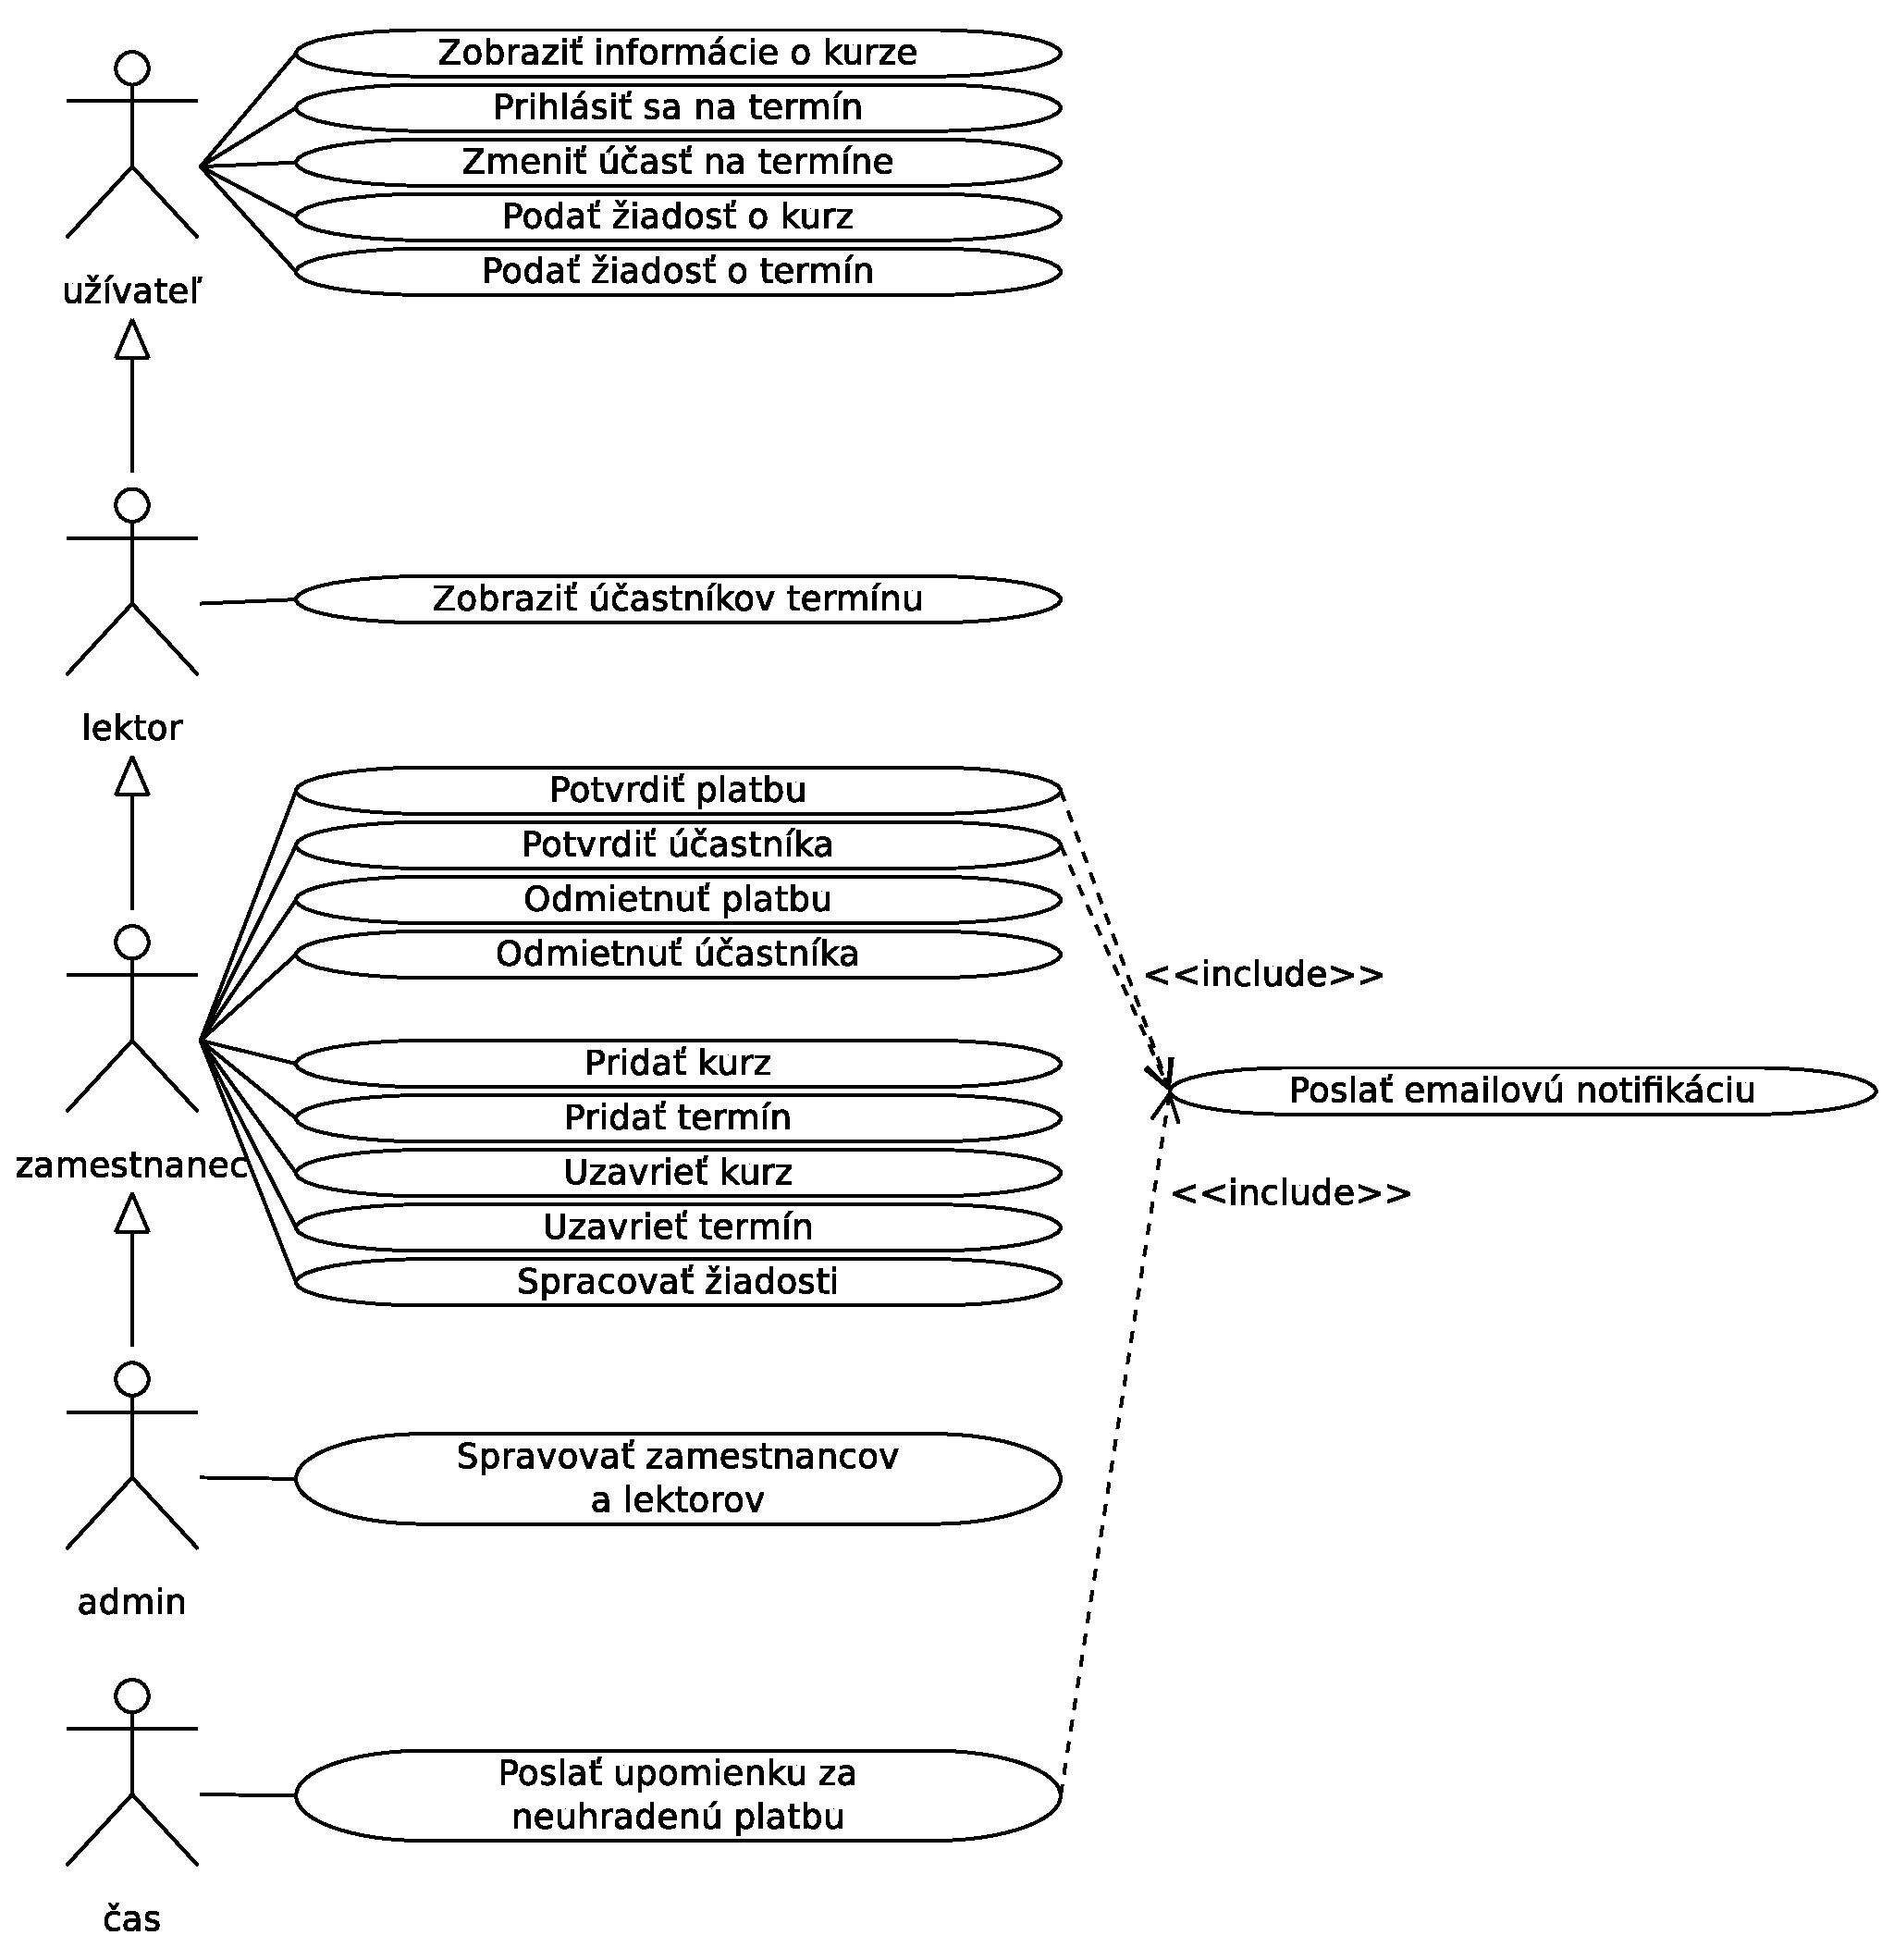
\includegraphics[height=17cm]{img/use_case_iter3.eps}
			\captionof{figure}{Diagram implementovaných případů použití po 3. iteraci.}
		\end{center}
		
Ve 3. iteraci by měl být zákazník spokojený s celkovou funkčností prototypu a ten se začne překlápět na již konečnou implementaci. Zároveň je přidána možnost žádosti o vypsání kursu/termínu a správy vlastní přihlášky.
	
	\subsubsection{4. iterácia}
		\begin{center}
			\captionsetup{type=figure}
			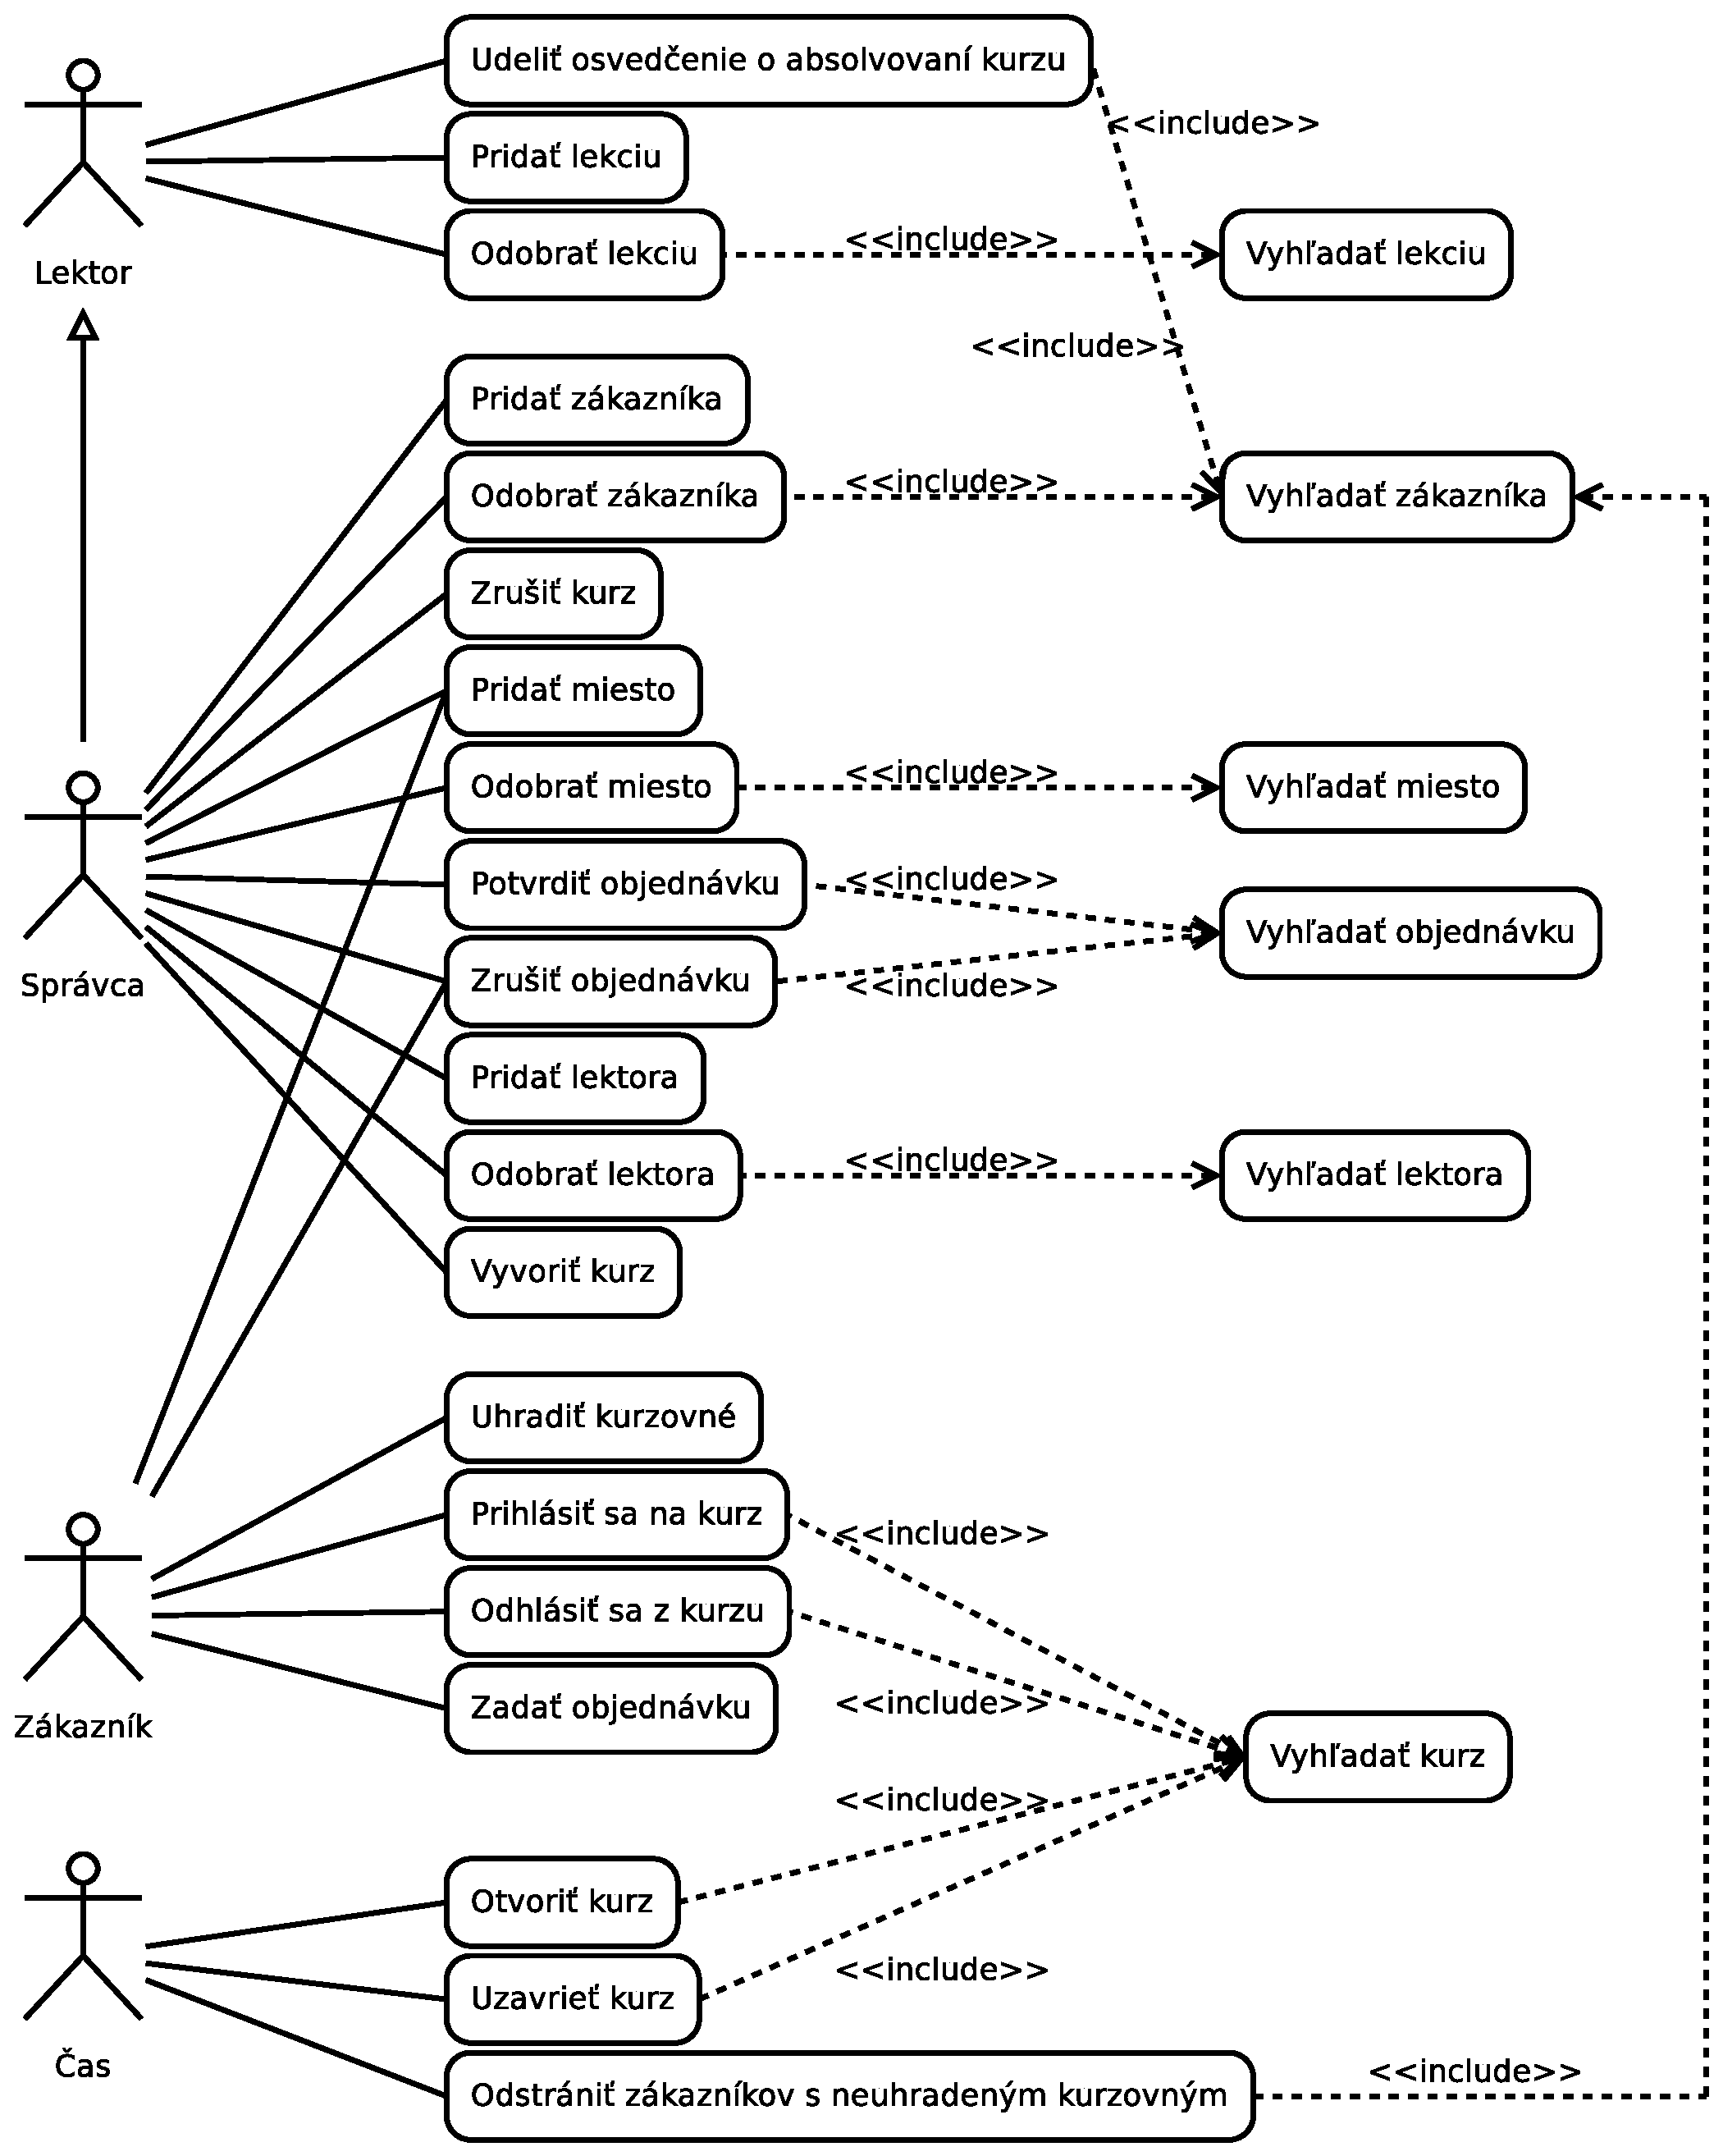
\includegraphics[height=17cm]{img/use_case.eps}
			\captionof{figure}{Diagram implementovaných případů použití po 4. iteraci.}
		\end{center}
		
Ve 4. iteraci se implementuje kalendář a evidence vrácených plateb. Jedná se především o detaily usnadňující práci se systémem, nikoliv už samotnou funkčnost.




%%%%%%%%%%%%%%%%%%%%%%%%%%%%%%%%%%%%%%%%%%%%%%%%%%%%%%
%------------------- 1. ITERACE ---------------------%
%%%%%%%%%%%%%%%%%%%%%%%%%%%%%%%%%%%%%%%%%%%%%%%%%%%%%%

\chapter{Modely - 1. iterace}

\section{UC1: Přidat termín}

V případě, že je již vytvořen kurz, je ke každému kurzu možnost vytvářet libovolný počet termínů. Termínem je myšlen konkrétní běh kurzu, který má daného lektora, probíhá v určitém časovém úseku (i více dní) a na určitém místě.

\begin{table}[h!]
	\begin{center}
    \begin{tabular}{ | p{4.2cm} | p{12.2cm} | }
    \hline
    \textbf{Název} & Přidat termín 
    \\ \hline
    
	\textbf{ID} & UC1
	\\ \hline
	
	\textbf{Popis} & Ke danému kurzu se vytvoří termín, tj. časový rozsah, kdy bude probíhat výuka daného kurzu. 
	\\ \hline
	    
	\textbf{Primární aktéři} & Zaměstnanec
	\\ \hline
	
	\textbf{Předpoklady} & Vybrán existující kurz
    \\ \hline                
    
    \textbf{Hlavní tok} &
    \vspace{-3.5mm}    
    \begin{enumerate}
    	\itemsep0em 
    	\item Zaměstnanec má vybraný konkrétní kurz a zde vybere "Přidat termín"
	    \item Zaměstnanec vyplní formulář a klikne na "Přidat"  	
	  	\item Systém ověří správně zadané údaje
	  	\begin{enumerate}
		  	\itemsep0em 
	  		\item Provede se kontrola správně zadaných formátů adresy, termínů začátku a konce, ceny, kapacity
	  		\item Provede se kontrola údajů na straně serveru
	  		\begin{enumerate}
			  	\itemsep0em 
	  			\item Termín konce nepředbíhá termín začátku
	  			\item Vybraný lektor nemá v daný termín nějaký jiný kurz
	  		\end{enumerate}
		\end{enumerate}
	    \item Systém přidá nový termín 
	    \item Systém zaměstnanci oznámí, že byl úspěšně zadán nový termín
	\end{enumerate}     
    \\ \hline
    
    \textbf{Výjimky} & 
    \vspace{-3.5mm}
    \begin{enumerate}
		\itemsep0em 
		\item Chybný vstup (UC1.1)
		\item Obsazený lektor (UC1.2)
	\end{enumerate}
    \\ \hline 
        
    \textbf{Následné podmínky} & Přidán termín ke kurzu
    \\ \hline    
    
	\textbf{Frekvence} & Několikrát za týden
	\\ \hline		
    \end{tabular}
	\end{center}	
	\caption{Specifikace hlavního toku Přidání termínu - UC1}  
\end{table}

\newpage

\subsection{Výjimka: Přidat termín - chybný vstup}

\begin{table}[!h]
	\begin{center}
    \begin{tabular}{ | p{4.2cm} | p{12.2cm} | }
    \hline
    \textbf{Název} & Přidat termín - chybný vstup
    \\ \hline
    
	\textbf{ID} & UC1.1
	\\ \hline
	
	\textbf{Popis} & Systém zaměstnanci oznámí, že zadal nesprávné údaje
	\\ \hline
	    
	\textbf{Primární aktéři} & Zaměstnanec
	\\ \hline
	
	\textbf{Předpoklady} & Zaměstnanec zadal nesprávně některý z údajů: adresa, termín začátku a konce, cena, kapacita
    \\ \hline
    
    \textbf{Alternativní tok} & 
    \vspace{-3.5mm}
    \begin{enumerate}
        \itemsep0em 
    	\item Spustí se po kroku 3(a). hlavního toku UC1 (ověření formátu zadaných údajů)
    	\item Systém zaměstnanci zobrazí, které formulářové prvky nesplňují validační kritéria
    \end{enumerate}
    \\ \hline  
    
	\textbf{Frekvence} & Často při vkládání termínu
	\\ \hline
	\end{tabular}
		\caption{Specifikace alternativního toku Přídání termínu - UC1.1 při chybném vstupu}	
	\end{center}
\end{table}

\subsection{Výjimka: Přidat termín - obsazený lektor}
\begin{table}[!h]	
	\begin{center}
    \begin{tabular}{ | p{4.2cm} | p{12.2cm} | }
    \hline
    \textbf{Název} & Přidat termín: obsazený lektor
    \\ \hline
    
	\textbf{ID} & UC1.2
	\\ \hline
	
	\textbf{Popis} & Systém zaměstnanci oznámí, že vybraný lektor je již obsazen
	\\ \hline
	    
	\textbf{Primární aktéři} & Zaměstnanec
	\\ \hline
	
	\textbf{Předpoklady} & Lektor má v daný termín, termín jiného kurzu
    \\ \hline
    
    \textbf{Alternativní tok} & 
	    \vspace{-3.5mm}
    	\begin{enumerate}
   	        \itemsep0em 
    		\item Spustí se po kroku 3(b)ii hlavního toku UC2 (ověření termínu a lektora)
	    	\item Systém přesměruje zaměstnance na předvyplněný formulář
	    	\item Systém zaměstnanci oznámí ať změní lektora nebo čas
    	\end{enumerate}
    \\ \hline 

	\textbf{Frekvence} & Vzácně při vkládání termínu
	\\ \hline
	\end{tabular}	
	\caption{Specifikace alternativního toku Přídání termínu - UC1.2 v případě, že je v daný termín obsazený lektor}	
	\end{center}
\end{table}

\newpage

\section{UC2: Přihlášení na termín}
Je-li k danému kurzu vypsán termín, mohou se na něj hlásit jak uživatelé, tak i neregistrovaní uživatelé.
\begin{table}[!h]
\begin{center}
    \begin{tabular}{ | p{4.2cm} | p{12.2cm} | }
    \hline
    \textbf{Název} & Přihlášení na termín 
    \\ \hline
    
	\textbf{ID} & UC2
	\\ \hline
	
	\textbf{Popis} & Vytvoří se přihláška na termín daného kurzu
	\\ \hline
	    
	\textbf{Primární aktéři} & Uživatel, neregistrovaný uživatel
	\\ \hline
	
	\textbf{Předpoklady} & 
	\vspace{-3.5mm}
	\begin{enumerate}
		\itemsep0em 	
		\item Vybrán vypsaný kurz
		\item Kurz má aspoň 1 vypsaný termín - je zobrazen přihlašovací formulář
	\end{enumerate}
    \\ \hline
    
    \textbf{Hlavní tok} & 
    \vspace{-3.5mm}
	\begin{enumerate}
		\itemsep0em 	
		\item Uživatel vyplní přihlašovací formulář a zvolí "Přihlásit"
		\item Provede se kontrola správně zadaných formátů a povinných položek: adresa, telefon, email, jméno, příjmení
		\item Provede se serverová kontrola
		\begin{enumerate}
			\itemsep0em 		
			\item Přihlašování na termín kurzu je otevřeno
			\item Přihláška již neexistuje - stejné jméno, příjmení a email
		\end{enumerate}				
		\item Vytvoří se registrace na daný termín
		\begin{enumerate}
			\itemsep0em 		
			\item Systém zkontroluje, zda-li je uživatel přihlášen
			\item Pokud ano, přidá k registraci ID uživatele
		\end{enumerate}				
		\item Systém na zadaný email odešle potvrzení o úspěšné registrace
	\end{enumerate}   		
    \\ \hline
    	   
    \textbf{Výjimky} & 
    \vspace{-3.5mm}
    \begin{enumerate}
	    \itemsep0em
     	\item Chybný vstup (UC2.1)
	    \item Uzavřené přihlašování (UC2.2)
    	\item Existující přihláška (UC2.3)
	    \item Chyba při odeslání potvrzovacího emailu (UC2.4)
    \end{enumerate}
	   
    \\ \hline
    
    \textbf{Následné podmínky} & Vytvořena registrace na daný termín kurzu
    \\ \hline        
    
	\textbf{Frekvence} & Několikrát denně
	\\ \hline
		
    \end{tabular}
	\caption{Specifikace hlavního toku Přihlášení na termín - UC2}    
	\end{center}

\end{table}

\newpage

\subsection{Výjimka: Přihlášení na termín - chybný vstup}

\begin{table}[!h]
	\begin{center}
    \begin{tabular}{ | p{4.2cm} | p{12.2cm} | }
    \hline
    \textbf{Název} & Přihlášení na termín - chybný vstup
    \\ \hline
    
	\textbf{ID} & UC2.1
	\\ \hline
	
	\textbf{Popis} & Systém uživateli oznámí, že zadal nesprávné údaje
	\\ \hline
	    
	\textbf{Primární aktéři} & Uživatel, neregistrovaný uživatel
	\\ \hline
	
	\textbf{Předpoklady} & Uživatel nebo neregistrovaný uživatel zadal nesprávně některý z údajů: adresa, telefon, email, jméno, příjmení
    \\ \hline
    
    \textbf{Alternativní tok} & 
    \vspace{-3.5mm}
    \begin{enumerate}
        \itemsep0em 
    	\item Spustí se po kroku 2. hlavního toku UC2 (ověření formátu zadaných údajů)
    	\item Systém zaměstnanci zobrazí, které formulářové prvky nesplňují validační kritéria
    \end{enumerate}
    \\ \hline              
    
	\textbf{Frekvence} & Často při podávání přihlášky
	\\ \hline
	\end{tabular}
		\caption{Výjimka Přihlášení na termín - UC2.1 při chybném vstupu}	
	\end{center}

\end{table}
\vspace{-0.5cm}
\subsection{Výjimka: Přihlášení na termín - uzavřené přihlašování}
\begin{table}[!h]
	\begin{center}
    \begin{tabular}{ | p{4.2cm} | p{12.2cm} | }
    \hline
    \textbf{Název} & Přihlášení na termín: uzavřený termín během přihlašování
    \\ \hline
    
	\textbf{ID} & UC2.2
	\\ \hline
	
	\textbf{Popis} & Systém uživateli oznámí, že termín je již uzavřen pro přihlašování. Tato situace může nastat v případě, že zaměstnanec uzavře přihlašování na kurz ve chvíli, kdy se na něj někdo hlásil.
	\\ \hline
	    
	\textbf{Primární aktéři} & Uživatel, neregistrovaný uživatel
	\\ \hline
	
	\textbf{Sekundární aktéři} & Zaměstnanec   
	\\ \hline
	
	\textbf{Předpoklady} & Termín kurzu je uzavřen pro přihlašování
    \\ \hline    
        
    \textbf{Akce pro spuštění} & Uživatel podá přihlášku a termín na který se hlásí je již uzavřen.
    \\ \hline
    
    \textbf{Alternativní tok} & 
    \vspace{-3.5mm}
	\begin{enumerate}
        \itemsep0em 	
		\item Spustí se po kroku 3(a) UC2 (kontrola, zda-li je otevřeno přihlašování)
		\item Systém uživatele přesměruje na stránku s daným kurzem
		\item Systém uživateli oznámí, že daný termín byl právě uzavřen
		\item Systém vykreslí přihlašovací formulář v případě, že je vypsán aspoň jeden termín
		\item Uživatel pokračuje krokem 1 UC2 (vyplnění formuláře)
	\end{enumerate}	     
    \\ \hline    
    
	\textbf{Frekvence} & Velmi vzácně při podávání přihlášky
	\\ \hline
	\end{tabular}
		\caption{Výjimka Přihlášení na termín - UC2.2 při uzavřeném přihlašování}
	\end{center}

\end{table}

\newpage

\subsection{Výjimka: Přihlášení na termín - existující přihláška}
\begin{table}[!h]
	\begin{center}
    \begin{tabular}{ | p{4.2cm} | p{12.2cm} | }
    \hline
    \textbf{Název} & Přihlášení na termín: existující přihláška
    \\ \hline
    
	\textbf{ID} & UC2.3
	\\ \hline
	
	\textbf{Popis} & Systém uživateli oznámí, že přihláška již existuje
	\\ \hline
	    
	\textbf{Primární aktéři} & Uživatel, neregistrovaný uživatel
	\\ \hline
	
	
	\textbf{Předpoklady} & Přihláška obsahující kombinaci jména, příjmení a emailu, která již existuje
    \\ \hline    
               
    \textbf{Alternativní tok} & 
    \vspace{-3.5mm}
	\begin{enumerate}
        \itemsep0em 	
		\item Spustí se po kroku 3(b) UC2 (kontrola existující přihlášky)
		\item Systém uživatele přesměruje na stránku s daným kurzem a předvyplněným formulářem
		\item Systém uživateli oznámí, že přihláška již existuje
	\end{enumerate}	     
    \\ \hline    
    
	\textbf{Frekvence} & Občas při podávání přihlášky
	\\ \hline
	\end{tabular}
		\caption{Výjimka Přihlášení na termín - UC2.3 při již existující registraci}
	\end{center}

\end{table}
\vspace{-0.5cm}
\subsection{Výjimka: Přihlášení na termín - chyba při odeslání potvrzovacího emailu}
\begin{table}[!h]
\begin{center}
    \begin{tabular}{ | p{4.2cm} | p{12.2cm} | }
    \hline
    \textbf{Název} & Přihlášení na termín: chyba při odeslání potvrzovacího emailu
    \\ \hline
    
	\textbf{ID} & UC2.4
	\\ \hline
	
	\textbf{Popis} & Dojde k chybě při posílání potvrzovacího emailu
	\\ \hline
	    
	\textbf{Primární aktéři} & Systém
	\\ \hline
	
	\textbf{Sekundární aktéři} & Uživatel, neregistrovaný  uživatel
	\\ \hline
	
	\textbf{Předpoklady} & 
    \vspace{-3.5mm}
	\begin{enumerate}
        \itemsep0em 		
		\item Přihláška byla úspěšně zpracována
		\item Systém se pokusí odeslat potvrzovací email o přihlášení na kurz		
	\end{enumerate}
    \\ \hline
    
    \textbf{Následné podmínky} & Email se vloží do fronty neodeslaných emailů
    \\ \hline 
    
    \textbf{Alternativní tok} & 

        \vspace{-3.5mm}  
		\begin{enumerate}
	        \itemsep0em 			
			\item Spustí se po kroku 5 UC2 (odeslání potvrzovacího emailu)
			\item Systému se nepodaří navázat spojení se SMTP serverem nebo SMTP server vrátí chybu, že se mu nepovedlo odeslat email
			\item Email se zařadí do fronty neodeslaných emailů
		\end{enumerate}		       
    \\ \hline    
    
	\textbf{Frekvence} & Velmi vzácně při podávání přihlášky
	\\ \hline
	\end{tabular}
\end{center}
	\caption{Výjimka Přihlášení na termín - UC2.4 dojde-li na chybu při odesílání potvrzovacího email}
\end{table}

\newpage

\section{UC3: Uzavření termínu}

Zaměstnanec může uzavírat a otevírat termíny. V případě, že je naplněna kapacita termínu nebo zaměstnanec tak sám usoudí, může přihlašování na daný termín uzavřít.


\begin{table}[!h]
\begin{center}
    \begin{tabular}{ | p{4.2cm} | p{12.2cm} | }
    \hline
    \textbf{Název} & Uzavření termínu
    \\ \hline
    
	\textbf{ID} & UC3
	\\ \hline
	
	\textbf{Popis} & Uzavření přihlašování na konkrétní termín
	\\ \hline
	    
	\textbf{Primární aktéři} & Zaměstnanec
	\\ \hline	
	
	\textbf{Předpoklady} & 
	\vspace{-3.5mm}
	\begin{enumerate}
        \itemsep0em 
		\item Vybrán termín kurzu
		\item Přihlašování na daný termín je otevřeno
	\end{enumerate}
    \\ \hline
    
    \textbf{Hlavní tok} & 
    \vspace{-3.5mm}
    \begin{enumerate}
        \itemsep0em     
    	\item Uživatel vybere "Uzavřít přihlašování" pro daný termín
    	\item Systém uzavře přihlašování pro daný termín
    \end{enumerate}
    \\ \hline
    
    \textbf{Následné podmínky} & Uzavřeno přihlašování na daný termín
    \\ \hline 
    
    \textbf{Výjimky} &
    žádné
    \\ \hline       
    
	\textbf{Frekvence} & Několikrát týdně
	\\ \hline
	
    \end{tabular}
\end{center}
\caption{Specifikace hlavního toku Užavření termínu - UC3}
\end{table}

\section{Konceptuální diagram tříd}

		% ----------- konceptualny diagram tried -----------
		\begin{center}
			\captionsetup{type=figure}
			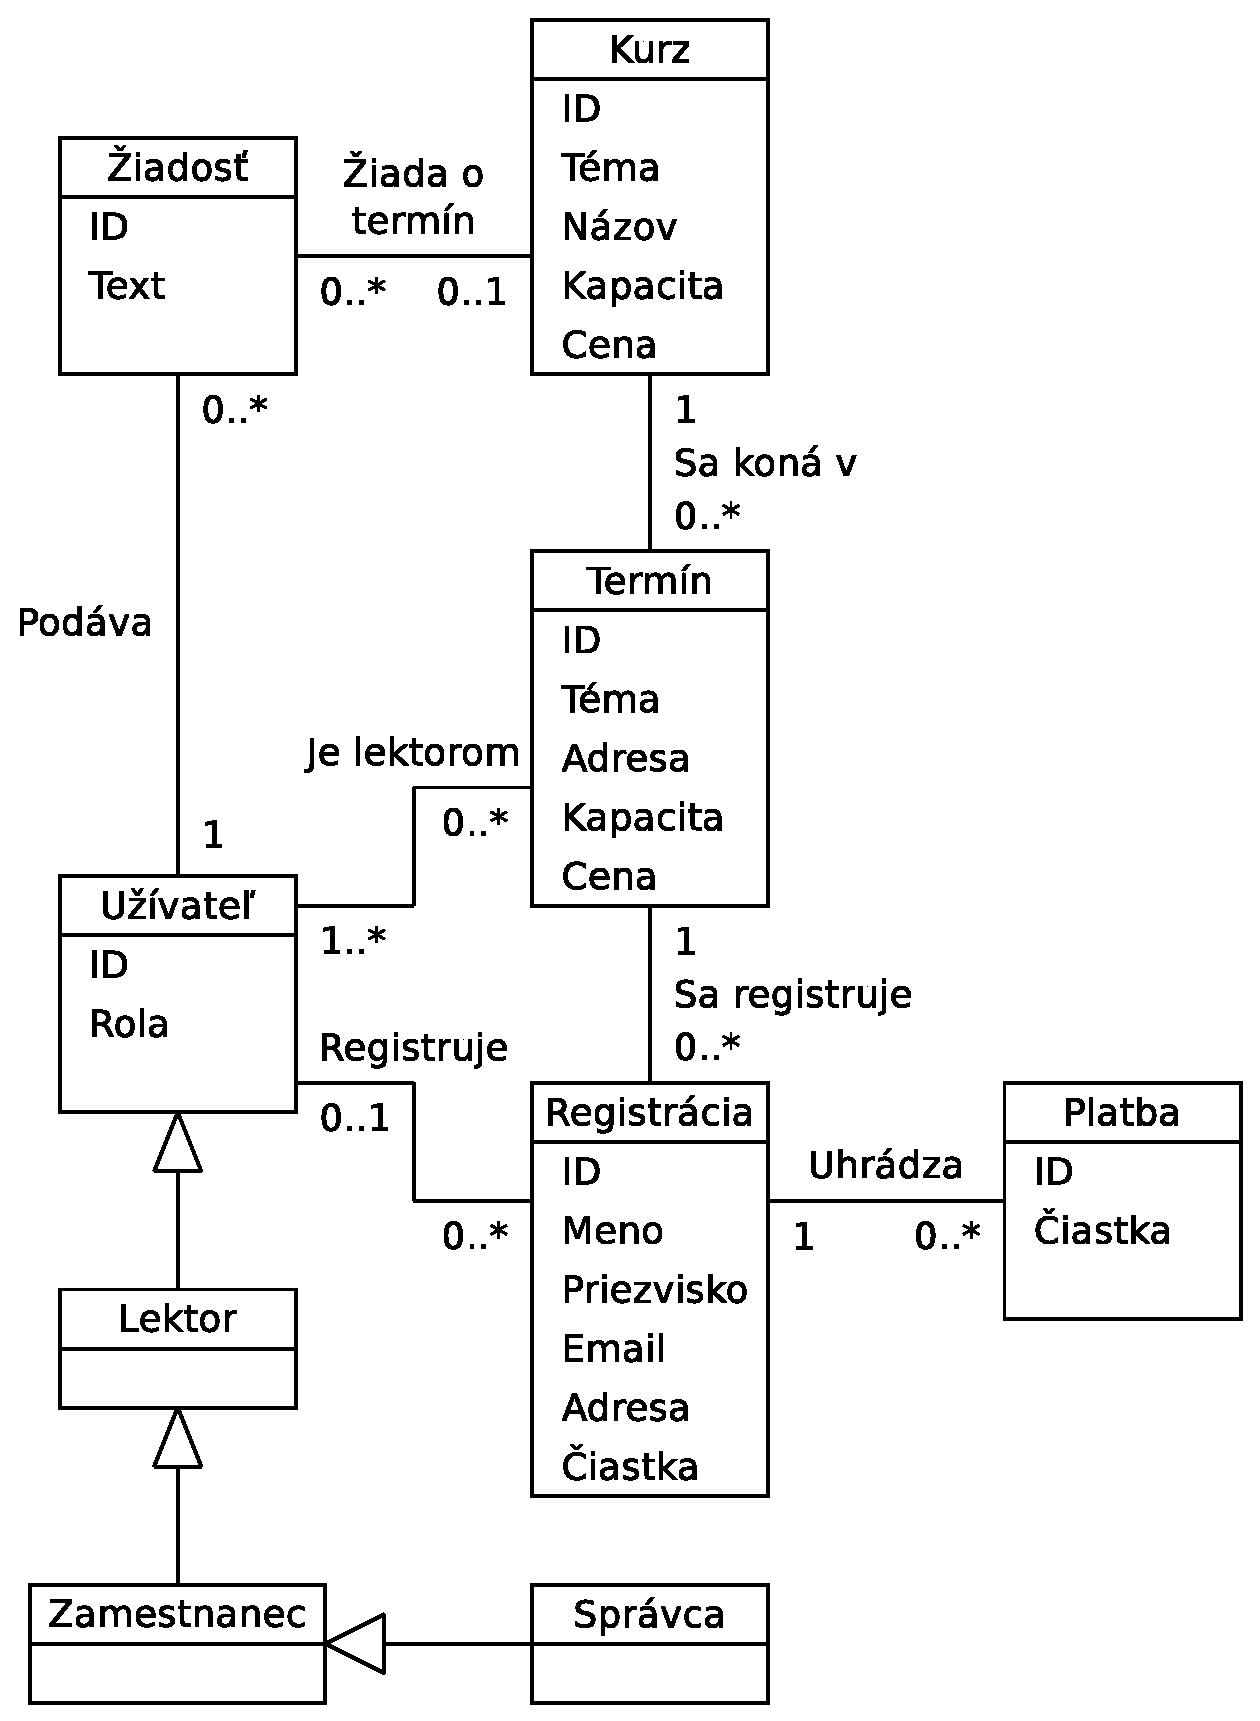
\includegraphics[height=17cm]{img/konceptualny_diagram_tried.eps}
			\captionof{figure}{Konceptuálny diagram tried po 1. iterácii.}
		\end{center}
		
	
		\section{Schéma návrhu databáze}
		% ----------- schema DB -----------
		\begin{center}
			\captionsetup{type=figure}
			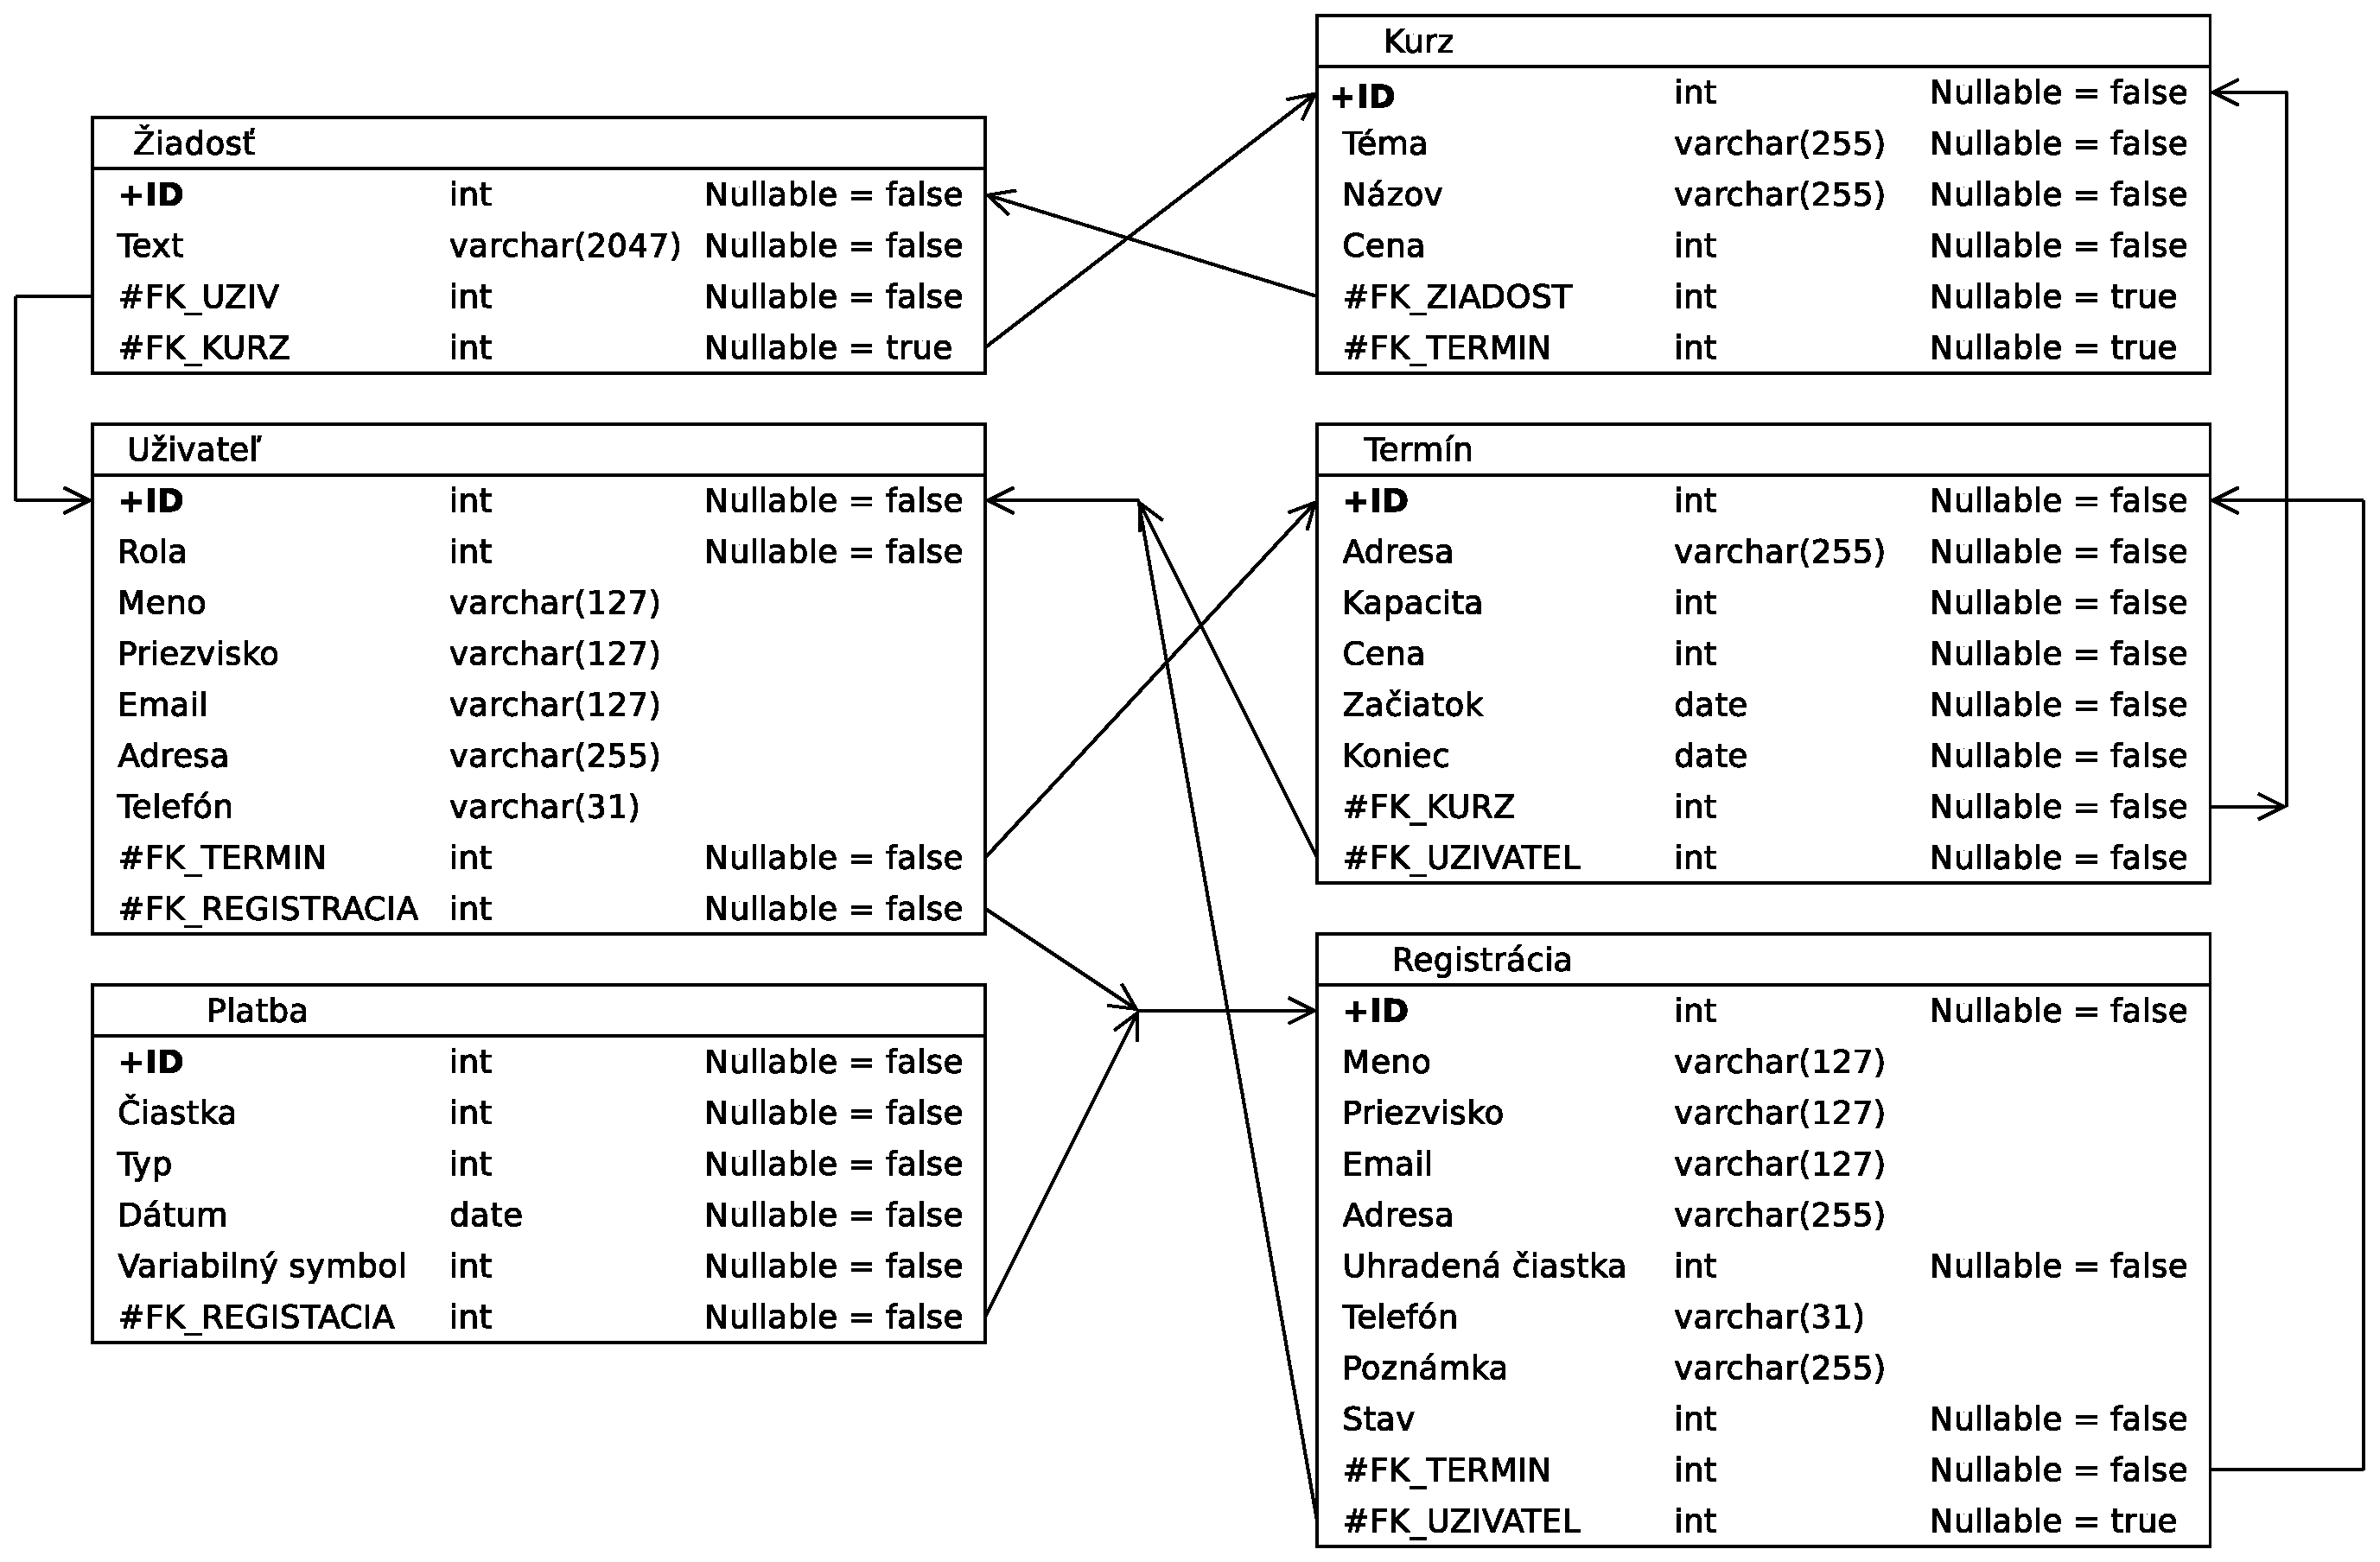
\includegraphics[height=12cm]{img/schema_db.eps}
			\captionof{figure}{Databázová schéma po 1. iterácii.}
		\end{center}				
		
		% ----------- architektura  -----------
		\section{Návrh architektury}				
		\begin{center}
			\captionsetup{type=figure}
			\includegraphics[width=18cm]{img/architektura-navrh.pdf}
			\captionof{figure}{Návrh architektury aplikace}
		\end{center}
		
		\paragraph{Poznámka:}
		HTTP požadavek je zpracováván Controllerem, který na jeho základě komunikuje s modelem a upravuje view.		

		
%%%%%%%%%%%%%%%%%%%%%%%%%%%%%%%%%%%%%%%%%%%%%%%%%%%%%%
%----------------- VÝSLEDNÉ MODELY ------------------%
%%%%%%%%%%%%%%%%%%%%%%%%%%%%%%%%%%%%%%%%%%%%%%%%%%%%%%		

\chapter{Výsledné modely analýzy a návrhu} 
\vspace{-0.5cm}
\section{UC4: Poslat upomínku za neuhrazenou platbu}
\begin{table}[h!]
	\begin{center}
    \begin{tabular}{ | p{4.2cm} | p{12.2cm} | }
    \hline
    \textbf{Název} & Poslat upomínku za neuhrazenou platbu
    \\ \hline
    
	\textbf{ID} & UC4
	\\ \hline
	
	\textbf{Popis} & Zkontrolují se nezaplacené přihlášky a rozešlou se upomínky
	\\ \hline
	    
	\textbf{Primární aktéři} & Systém
	\\ \hline
	
	\textbf{Předpoklady} & -
    \\ \hline                
    
    \textbf{Hlavní tok} &
    \vspace{-3.5mm}    
    \begin{enumerate}
    	\itemsep0em 
    	\item Systém zkontroluje všechny nezaplacené přihlášky na kurzy probíhající od aktuálního data do budoucnosti
    	\item Zkontroluje se počet již odeslaných upomínek
	    \item Vypočte se časový rozdíl mezi datem přihlášky a aktuálním časem
	    \begin{enumerate}
		    \itemsep0em
	    	\item Pokud časový rozdíl je větší než počet dní uveden v konfiguraci pro 1. upomínku a ta ještě nebyla odeslána, pošle se 1. upomínka
	    	\item Pokud časový rozdíl je větší než počet dní uveden v konfiguraci pro 2. upomínku a ta ještě nebyla odeslána, pošle se 2. upomínka
   		    \item Na základě nastavení v konfiguraci. Pokud je časový rozdíl větší, než počet dní pro zaslání návrhu na vyřazení a již uplynul dostatečný počet dní od posledního zaslání, pošle se email s návrhem na vyřazení na daný email
   		    \begin{enumerate}
	   		    \itemsep0em
   		    	\item Registrace se v databázi označí jako navržená k vyřazení
   		    \end{enumerate}
	    \end{enumerate}
	    \item Zaznamená se odeslání upomínky	 
	\end{enumerate}     
    \\ \hline
    
    \textbf{Výjimky} & 
    \vspace{-3.5mm}
    \begin{enumerate}
		\itemsep0em 
		\item Chyba při odeslání emailu
	\end{enumerate}
    \\ \hline 
        
    \textbf{Následné podmínky} & Upomínka odeslána
    \\ \hline    
    
	\textbf{Frekvence} & Každý den
	\\ \hline		
    \end{tabular}
	\end{center}	
	\caption{Specifikace hlavního toku Posílání upomínek - UC4}  
\end{table}

\newpage



\section{UC5: Potvrzení/odmítnutí/vyřazení přihlášky/platby}

V seznamu registrací je možné přecházet mezi jednotlivými stavy po kliknutí na příslušná tlačítka. Např. registraci ve stavu \verb|POTVRZENA| můžeme po kliknutí na tlačítko "vyřadit" změnit na \verb|VYRAZENA| nebo po kliknutí na "potvrdit platbu" na \verb|ZAPLACENA|. Nejlépe vše popisuje následující stavový diagram.

\begin{center}
	\captionsetup{type=figure}
	\includegraphics[width=10cm]{img/prihlaska-stavy.pdf}
	\captionof{figure}{Stavy přihlášky}
\end{center}

\begin{table}[h!]
	\begin{center}
    \begin{tabular}{ | p{4.2cm} | p{12.2cm} | }
    \hline
    \textbf{Název} & Potvrzení/Odmítnutí/Vyřazení přihlášky
    \\ \hline
    
	\textbf{ID} & UC5a
	\\ \hline
	
	\textbf{Popis} & V seznamu registrací je možné přecházet mezi stavy jednotlivých registrací. Nejlépe vše popisuje výše přiložený stavový diagram.
	\\ \hline
	    
	\textbf{Primární aktéři} & Zaměstnanec, Admin
	\\ \hline
	
	\textbf{Předpoklady} & 
	\vspace{-3.5mm}  
	\begin{enumerate}
		\itemsep0em
		\item Uživatel přihlášen jako Zaměstnanec nebo Admin
	\end{enumerate}
    \\ \hline                
    
    \textbf{Hlavní tok} &
    \vspace{-3.5mm}    
    \begin{enumerate}
    	\itemsep0em 
    	\item Uživatel klikne na příslušné tlačítko (viz. název přechodu ve stavovém diagramu)
    	\item Systém změní stav přihlášky
    	\item Systém pošle upozornění na email zadaný u registrace 
	\end{enumerate}     
    \\ \hline
    
    \textbf{Výjimky} & 
    \vspace{-3.5mm}
    \begin{enumerate}
		\itemsep0em 
		\item Chyba při odeslání emailu
	\end{enumerate}
    \\ \hline 
        
    \textbf{Následné podmínky} & Stav registrace změněn
    \\ \hline    
    
	\textbf{Frekvence} & Každý den
	\\ \hline		
    \end{tabular}
	\end{center}	
	\caption{Specifikace hlavního toku změny stavu přihlášky - UC5a}  
\end{table}


\begin{table}[h!]
	\begin{center}
    \begin{tabular}{ | p{4.2cm} | p{12.2cm} | }
    \hline
    \textbf{Název} & Potvrzení platby
    \\ \hline
    
	\textbf{ID} & UC5b
	\\ \hline
	
	\textbf{Popis} & Potvrzení platby. Kurz může být zaplacen celý a nebo jen z části.
	\\ \hline
	    
	\textbf{Primární aktéři} & Zaměstnanec, Systém
	\\ \hline
	
	\textbf{Předpoklady} & 
    \vspace{-3.5mm} 	
	\begin{enumerate}
		\itemsep0em
		\item Uživatel přihlášen jako Zaměstnanec nebo Admin
		\item Registrace je ve stavu \verb|POTVRZENA|
	\end{enumerate}
    \\ \hline            
    
    \textbf{Hlavní tok} &
    \vspace{-3.5mm}    
    \begin{enumerate}
    	\itemsep0em 
    	\item Uživatel klikne na tlačítko "Potvrdit platbu"
    	\item Systém vyvolá modální okno s formulářem pro evidenci platby
    	\item Uživatel vyplní formulář a odešlo ho
		\item Systém vloží platbu do databáze 	
		\begin{enumerate}
			\itemsep0em 		
			\item Platba je částečná
			\begin{enumerate}
				\itemsep0em 					
				\item Systém odečte platbu od celkové ceny registrace
			\end{enumerate}
			\item Platba je celá nebo se jedná o zbytek celkové ceny
			\begin{enumerate}
				\itemsep0em 			
				\item Systém odečte platbu od celkové ceny registrace
				\item Systém změní stav registrace na \verb|ZAPLACENA|
			\end{enumerate}
	    \end{enumerate}
    	\item Systém pošle upozornění na email zadaný u registrace 	 
	\end{enumerate}     
    \\ \hline
    
    \textbf{Výjimky} & 
    \vspace{-3.5mm}
    \begin{enumerate}
		\itemsep0em 
		\item Chyba při odeslání emailu
		\item Platba je větší, než-li zbývající částka
	\end{enumerate}
    \\ \hline 
        
    \textbf{Následné podmínky} & Upomínka odeslána
    \\ \hline    
    
	\textbf{Frekvence} & Každý den
	\\ \hline		
    \end{tabular}
	\end{center}	
	\caption{Specifikace hlavního toku potvrzení platby - UC5b}  
\end{table}

\newpage

\section{Volba frameworku}

Framework pro realizaci architektury jsme zvolili Play! pro Javu (\href{http://www.playframework.com/}{http://www.playframework.com/}), který již v sobě zahrnuje šablonovací systém pro tvorbu jednotlivých Views a základní třídy pro Controller a Model.

\section{Finální diagram tříd}
		
\begin{center}
	\captionsetup{type=figure}
	\includegraphics[height=22cm]{img/architektura-detail.pdf}
	\captionof{figure}{Návrh finálního diagramu tříd}
\end{center}	


		% ----------- interakce  -----------
		
\section{Diagramy sekvence a komunikace}

\begin{center}
	\captionsetup{type=figure}
	\includegraphics[height=11cm]{img/uc1-pridat-termin.pdf}
	\captionof{figure}{Sekvenční diagram UC1 Přidání termínu}
\end{center}

\begin{center}
	\captionsetup{type=figure}
	\includegraphics[height=10cm]{img/uc3-uzavrit-termin.pdf}
	\captionof{figure}{Sekvenční diagram UC3 Uzavření termínu}
\end{center}

\begin{center}
	\captionsetup{type=figure}
	\includegraphics[width=15.5cm]{img/uc2-prihlaseni-na-termin.pdf}
	\captionof{figure}{Sekvenční diagram UC2 Příhlášení na termín}
\end{center}

\begin{center}
	\captionsetup{type=figure}
	\includegraphics[width=15cm]{img/uc2-prihlaseni-na-termin-seq.pdf}
	\captionof{figure}{Diagram komunikace UC Příhlášení na termín}
\end{center}

\section{Interakce mezi obrazovkami}

\paragraph{Front End} je rozhraní se kterým můžou interagovat všichni uživatelé, ať už jsou registrovaní nebo ne a všichni ho vidí stejně. Slouží především pro prezentaci kurzů a registraci na jednotlivé termíny.

\begin{center}
	\captionsetup{type=figure}
	\includegraphics[width=18cm]{img/frontend-obr.pdf}
	\captionof{figure}{Interakce mezi obrazovkami - Front End / Klientská část}
\end{center}

\paragraph{Back End} je rozhraní se kterým můžou interagovat pouze Zaměstnanci a Adminové. Slouží ke správě termínů, kurzů a další administrační činnosti.

\begin{center}
	\captionsetup{type=figure}
	\includegraphics[width=17cm]{img/backend-obr.pdf}
	\captionof{figure}{Interakce mezi obrazovkami - Back End / Administrační rozhraní}
\end{center}
		
		
		


% ----------------- prejimaci testy ----------------- %
	
\section{Přejímací testy}

% ----------------- prihlaska na termin ----------------- %

\subsection{Přihláška na termín kurzu}

\paragraph{Popis}

Uživatel se přihlásí na konkrétní termín nějakého kurzu.

\paragraph{Předpoklady}

\begin{itemize}
	\item V databázi je uložen aspoň jeden kurz a k němu aspoň jeden termín
\end{itemize}

\paragraph{Postup}
\begin{enumerate}
	\item Uživatel zvolí detail kurzu (ze Seznamu kurzů nebo z Homepage)
	\item Uživatel vyplní registrační formulář a potvrdí registraci kliknutím na tlačítko
	\item Možné reakce:
	\begin{enumerate}
		\item \textcolor{LimeGreen}{Úspěch} - systém zaznamená registraci (uloží do databáze) a odešle potvrzovací email o přijetí registrace
		\item \textcolor{LimeGreen}{Úspěch} - systém zaznamená registraci (uloží do databáze), ale nepovede se odeslat potvrzovací email (email je uložen do fronty k odeslání)
		\item \textcolor{Red}{Chyba} - chybný vstup - systém označí chybný vstup
		\item \textcolor{Red}{Chyba} - uzavřené přihlašování - systém uživatele upozorní, že je přihlašování již uzavřené a přesměruje ho na tu samou stránku (zmizí přihlašovací formulář)
		\item \textcolor{Red}{Chyba} - existující přihláška (shoda jména, příjmení a emailu)
	\end{enumerate}
	\item Uživatel zkontroluje jím zadaný email, zda-li mu přišla potvrzovací zpráva o přijetí registrace
\end{enumerate}

% ----------------- vypsani noveho kurzu ----------------- %

\subsection{Vypsání nového kurzu}

\paragraph{Popis}

Uživatel (Zaměstnanec nebo Admin) přidá nový kurz.

\paragraph{Předpoklady}

\begin{itemize}
	\item Uživatel je přihlášen a má práva Zaměstnance nebo Admina
\end{itemize}

\paragraph{Postup}

\begin{enumerate}
	\item Uživatel zvolí "Přidat kurz" na obrazovce Seznamu kurzů
	\item Uživatel vyplní formulář a potvrdí jeho odeslání kliknutím na tlačítko
	\item Možné reakce:
	\begin{enumerate}
		\item \textcolor{LimeGreen}{Úspěch} - systém přidá nový kurz do databáze, oznámí uživateli, že byl nový kurz úspěšně přidán a přesměruje ho na seznam kurzů
		\item \textcolor{Red}{Chyba} - chybný vstup - systém označí chybný vstup
	\end{enumerate}	
\end{enumerate}


% ----------------- vypsani noveho terminu ----------------- %

\subsection{Vypsání nového termínu}

\paragraph{Popis}

Uživatel (Zaměstnanec nebo Admin) přidá nový termín pro daný kurz.

\paragraph{Předpoklady}

\begin{itemize}
	\item V databázi je uložen aspoň jeden kurz
	\item Uživatel je přihlášen a má práva Zaměstnance nebo Admina
\end{itemize}

\paragraph{Postup}

\begin{enumerate}
	\item Uživatel zvolí "Přidat termín" ze Seznamu termínu nebo Seznamu kurzů
	\item Uživatel vyplní formulář a potvrdí jeho odeslání kliknutím na tlačítko
	\item Možné reakce:
	\begin{enumerate}
		\item \textcolor{LimeGreen}{Úspěch} - systém přidá nový termín do databáze, oznámí uživateli, že byl nový termín úspěšně přidán a přesměruje ho na seznam termínů
		\item \textcolor{Red}{Chyba} - chybný vstup - systém označí chybný vstup
		\item \textcolor{Red}{Chyba} - obsazený lektor - systém upozorní uživatele, že daný lektor je již obsazený
	\end{enumerate}
\end{enumerate}

\end{document}


